\documentclass[a4paper,11pt,twoside]{report}
% THIS FILE SHOULD BE COMPILED BY pdfLaTeX

% ----------------------   PREAMBLE PART ------------------------------

% ------------------------ ENCODING & LANGUAGES ----------------------

\usepackage[utf8]{inputenc}
%\usepackage[MeX]{polski} % Not needed unless You have a name with polish symbols or sth
\usepackage[T1]{fontenc}
\usepackage[english, polish]{babel}


\usepackage{amsmath, amsfonts, amsthm, latexsym} % MOSTLY MATHEMATICAL SYMBOLS

\usepackage[final]{pdfpages} % INPUTING TITLE PDF PAGE - GENERATE IT FIRST!
%\usepackage[backend=bibtex, style=verbose-trad2]{biblatex}


\usepackage{commath} % various commands which can make writing math expressions easier --- documentation available at: https://ctan.gust.org.pl/tex-archive/macros/latex/contrib/commath/commath.pdf

\usepackage[hidelinks]{hyperref} % for hyperlinks, for example, urls, references to equations, entries in a bibliography --- hidelinks option removes rectangles around hiperlinks


% ---------------- MARGINS, INDENTATION, LINESPREAD ------------------

\usepackage[inner=20mm, outer=20mm, bindingoffset=10mm, top=25mm, bottom=25mm]{geometry} % MARGINS


\linespread{1.5}
\allowdisplaybreaks         % ALLOWS BREAKING PAGE IN MATH MODE

\usepackage{indentfirst}    % IT MAKES THE FIRST PARAGRAPH INDENTED; NOT NEEDED
\setlength{\parindent}{5mm} % WIDTH OF AN INDENTATION


%---------------- RUNNING HEAD - CHAPTER NAMES, PAGE NUMBERS ETC. -------------------

\usepackage{fancyhdr}
\pagestyle{fancy}
\fancyhf{}
% PAGINATION: LEFT ALIGNMENT ON EVEN PAGES, RIGHT ALIGNMENT ON ODD PAGES 
\fancyfoot[LE,RO]{\thepage} 
% RIGHT HEADER: zawartość \rightmark do lewego, wewnętrznego (marginesu) 
\fancyhead[LO]{\sc \nouppercase{\rightmark}}
% lewa pagina: zawartość \leftmark do prawego, wewnętrznego (marginesu) 
\fancyhead[RE]{\sc \leftmark}

\renewcommand{\chaptermark}[1]{\markboth{\thechapter.\ #1}{}}

% HEAD RULE - IT'S A LINE WHICH SEPARATES HEADER AND FOOTER FROM CONTENT
\renewcommand{\headrulewidth}{0 pt} % 0 MEANS NO RULE, 0.5 MEANS FINE RULE, THE BIGGER VALUE THE THICKER RULE


\fancypagestyle{plain}{
  \fancyhf{}
  \fancyfoot[LE,RO]{\thepage}
  
  \renewcommand{\headrulewidth}{0pt}
  \renewcommand{\footrulewidth}{0.0pt}
}



% --------------------------- CHAPTER HEADERS ---------------------

\usepackage{titlesec}
\titleformat{\chapter}
  {\normalfont\Large \bfseries}
  {\thechapter.}{1ex}{\Large}

\titleformat{\section}
  {\normalfont\large\bfseries}
  {\thesection.}{1ex}{}
\titlespacing{\section}{0pt}{30pt}{20pt} 

    
\titleformat{\subsection}
  {\normalfont \bfseries}
  {\thesubsection.}{1ex}{}


% ----------------------- TABLE OF CONTENTS SETUP ---------------------------

\def\cleardoublepage{\clearpage\if@twoside
\ifodd\c@page\else\hbox{}\thispagestyle{empty}\newpage
\if@twocolumn\hbox{}\newpage\fi\fi\fi}


% THIS MAKES DOTS IN TOC FOR CHAPTERS
\usepackage{etoolbox}
\makeatletter
\patchcmd{\l@chapter}
  {\hfil}
  {\leaders\hbox{\normalfont$\m@th\mkern \@dotsep mu\hbox{.}\mkern \@dotsep mu$}\hfill}
  {}{}
\makeatother

\usepackage{titletoc}
\makeatletter
\titlecontents{chapter}% <section-type>
  [0pt]% <left>
  {}% <above-code>
  {\bfseries \thecontentslabel.\quad}% <numbered-entry-format>
  {\bfseries}% <numberless-entry-format>
  {\bfseries\leaders\hbox{\normalfont$\m@th\mkern \@dotsep mu\hbox{.}\mkern \@dotsep mu$}\hfill\contentspage}% <filler-page-format>

\titlecontents{section}
  [1em]
  {}
  {\thecontentslabel.\quad}
  {}
  {\leaders\hbox{\normalfont$\m@th\mkern \@dotsep mu\hbox{.}\mkern \@dotsep mu$}\hfill\contentspage}

\titlecontents{subsection}
  [2em]
  {}
  {\thecontentslabel.\quad}
  {}
  {\leaders\hbox{\normalfont$\m@th\mkern \@dotsep mu\hbox{.}\mkern \@dotsep mu$}\hfill\contentspage}
\makeatother



% ---------------------- TABLES AD FIGURES NUMBERING ----------------------

\renewcommand*{\thetable}{\arabic{chapter}.\arabic{table}}
\renewcommand*{\thefigure}{\arabic{chapter}.\arabic{figure}}


% ------------- DEFINING ENVIRONMENTS FOR THEOREMS, DEFINITIONS ETC. ---------------

\makeatletter
\newtheoremstyle{definition}
{3ex}%                           % Space above
{3ex}%                           % Space below
{\upshape}%                      % Body font
{}%                              % Indent amount
{\bfseries}%                     % Theorem head font
{.}%                             % Punctuation after theorem head
{.5em}%                          % Space after theorem head, ' ', or \newline
{\thmname{#1}\thmnumber{ #2}\thmnote{ (#3)}}
\makeatother

\theoremstyle{definition}
\newtheorem{theorem}{Theorem}[chapter]
\newtheorem{lemma}[theorem]{Lemma}
\newtheorem{example}[theorem]{Example}
\newtheorem{proposition}[theorem]{Proposition}
\newtheorem{corollary}[theorem]{Corollary}
\newtheorem{definition}[theorem]{Definition}
\newtheorem{remark}[theorem]{Remark}

% --------------------- END OF PREAMBLE PART (MOSTLY) --------------------------





% -------------------------- USER SETTINGS ---------------------------

\usepackage{float}
\usepackage{listings}
\usepackage{xcolor}
\usepackage{menukeys}
\usepackage{array}

\lstdefinelanguage{json}{
    basicstyle=\normalfont\ttfamily,
    numbers=left,
    numberstyle=\scriptsize,
    stepnumber=1,
    numbersep=8pt,
    showstringspaces=false,
    breaklines=true,
    frame=lines,
    backgroundcolor=\color[rgb]{0.95, 0.95, 0.95},
    stringstyle=\color[rgb]{0.25,0.5,0.35},
    keywordstyle=\color[rgb]{0.5,0.0,0.35},
    commentstyle=\color[rgb]{0.5,0.5,0.5},
    string=[s]{"}{"},
    comment=[l]{//},
    morecomment=[s]{/*}{*/},
    tabsize=2,
    keywords={},
}

\newcommand{\tytul}{Proceduralne generowanie świata i wyzwania związane z renderowaniem w przestrzeniach nieeuklidesowych}
\renewcommand{\title}{Procedural world generation and the challenges of rendering in non-Euclidean spaces}
\newcommand{\type}{Engineer} % Master OR Engineer
\newcommand{\supervisor}{Paweł Kotowski, Ph.D.} % TITLE AND NAME OF THE SUPERVISOR



\begin{document}
\sloppy
\selectlanguage{english}


\includepdf[pages=-]{title_page} % THIS INPUTS THE TITLE PAGE

\null\thispagestyle{empty}\newpage

% ------------------ PAGE WITH SIGNATURES --------------------------------

%\thispagestyle{empty}\newpage
%\null
%
%\vfill
%
%\begin{center}
%\begin{tabular}[t]{ccc}
%............................................. & \hspace*{100pt} & .............................................\\
%supervisor's signature & \hspace*{100pt} & author's signature
%\end{tabular}
%\end{center}
%


% ---------------------------- ABSTRACTS -----------------------------

{  \fontsize{12}{14} \selectfont
\begin{abstract}

    \begin{center}
        \title
    \end{center}
    Procedural generation, as a method used in creating video games, has experienced a significant increase in popularity in recent years.
    It has been employed extensively in acclaimed titles such as \textit{Minecraft} and \textit{No Man's Sky} to create virtually infinite worlds that the player is free to interact with.
    On the other hand, a recent game \textit{Hyperbolica} popularized a novel idea of making the virtual worlds even more interesting by setting them in non-Euclidean spaces.
    This work describes the implementation of a video game that incorporates both of the aforementioned concepts.

    In the game, we use and expand on the technique of transforming Euclidean space into hyperbolic or spherical space introduced by László Szirmay-Kalos and Milán Magdics in \cite{Szirmay-Kalos2022}.
    The approach allows for the use of established algorithms, developed with Euclidean geometry in mind, in other geometries.
    %This approach also simplifies the implementation of the game logic in different geometries as large parts of the implementation can be shared across the three geometries.
    Furthermore, core parts of the game logic can be shared between different geometries, which vastly simplifies the implementation.
    The approach also allows for changing the degree to which the scene is visually curved in hyperbolic geometry at runtime.

    The procedural terrain generation in the game is based on the marching cubes algorithm with Perlin noise used for generating the underlying scalar field.

    The game also includes several classic game features, such as terrain editing, character animations, day/night cycle, and many more.
    As a result, the game offers a unique experience of exploring and interacting with worlds inherently different from the one we live in. \\

    \noindent \textbf{Keywords:} Non-Euclidean Geometry, Hyperbolic Geometry, Spherical Geometry, Procedural Generation, Video Games, OpenGL, C\#
    \question{Should keywords start with capital letters?}
\end{abstract}
}

\null\thispagestyle{empty}\newpage


{\selectlanguage{polish} \fontsize{12}{14}\selectfont
\begin{abstract}

    \begin{center}
        \tytul
    \end{center}
    Proceduralne generowanie świata jest techniką zdobywającą rosnącą popularność przy tworzeniu gier komputerowych.
    Zostało ono wykorzystane z powodzeniem m. in. w takich produkcjach jak \textit{Minecraft} czy \textit{No Man's Sky}.
    Z drugiej strony za przyczyną gier takich jak \textit{Hyperbolica}, szersze zainteresowanie zyskała kwestia osadzania gier komputerowych w przestrzeniach nieeuklidesowych.
    Niniejsza praca opisuje implementację gry komputerowej, która łączy oba te podejścia.

    W grze zastosowano, z pewnymi modyfikacjami, metodę przekształcania przestrzeni euklidesowej w przestrzeń hiperboliczną lub sferyczną, zaproponowaną przez László Szirmay-Kalosa i Milána Magdicsa w \cite{Szirmay-Kalos2022}.
    Wspomniane podejście pozwala na wykorzystanie znanych algorytmów, zaprojektowanych z myślą o geometrii euklidesowej w innych geometriach.
    Dodatkowo, kluczowe części logiki gry mogą być dzięki temu dzielone pomiędzy różnymi geometriami, co znacznie upraszcza implementację.
    Zastosowana metoda pozwala również na zmianę stopnia zakrzywienia sceny w czasie rzeczywistym w przestrzeni hiperbolicznej.

    Proceduralne generowanie terenu w grze opiera się na algorytmie maszerujących sześcianów (ang. \textit{marching cubes algorithm}) z polem skalarnym określonym za pomocą szumu Perlina.

    Gra zawiera również wiele klasycznych funkcjonalności, takich jak edycja terenu, animacje postaci, cykl dnia i nocy oraz wiele innych.
    W rezultacie gra oferuje unikalne doświadczenie eksploracji i interakcji z światami fundamentalnie różnymi od tego, w którym żyjemy. \\

    \noindent \textbf{Słowa kluczowe:} geometria nieeuklidesowa, geometria hiperboliczna, geometria sferyczna, proceduralne generowanie terenu, gry komputerowe, OpenGL, C\#
\end{abstract}
}


%% --------------------------- DECLARATIONS ------------------------------------
%
%%
%%	IT IS NECESSARY OT ATTACH FILLED-OUT AUTORSHIP DEECLRATION. SCAN (IN PDF FORMAT) NEEDS TO BE PLACED IN scans FOLDER AND IT SHOULD BE CALLED, FOR EXAMPLE, DECLARATION_OF_AUTORSHIP.PDF. IF THE FILENAME OR FILEPATH IS DIFFERENT, THE FILEPATH IN THE NEXT COMMAND HAS TO BE ADJUSTED ACCORDINGLY.
%%
%%	command attacging the declarations of autorship
%%
%\includepdf[pages=-]{scans/declaration-of-autorship}
%\null\thispagestyle{empty}\newpage
%
%% optional declaration
%%
%%	command attaching the declaataration on granting a license
%%
%\includepdf[pages=-]{scans/declaration-on-granting-a-license}
%%
%%	.tex corresponding to the above PDF files are present in the 3. declarations folder 
%
\null\thispagestyle{empty}\newpage
% ------------------- TABLE OF CONTENTS ---------------------
% \selectlanguage{english} - for English
\pagenumbering{gobble}
\tableofcontents
\thispagestyle{empty}
\newpage % IF YOU HAVE EVEN QUANTITY OD PAGES OF TOC, THEN REMOVE IT OR ADD \null\newpage FOR DOUBLE BLANK PAGE BEFORE INTRODUCTION


% -------------------- THE BODY OF THE THESIS --------------------------------

\null\thispagestyle{empty}\newpage
\pagestyle{fancy}
\pagenumbering{arabic}
\setcounter{page}{11}


\chapter{Introduction}\label{ch:introduction}
\markboth{}{Introduction}
\addcontentsline{toc}{chapter}{Introduction}

What is the thesis about? What is the content of it? What is the Author's contribution to it?
\par
WARNING!  In a diploma thesis which is a team project: Description of the work division in the team, including the scope of each co-author’s contribution to the practical part (Team Programming Project) and the descriptive part of the diploma thesis.
\par

Lorem ipsum dolor sit amet, consetetur sadipscing elitr, sed diam nonumyeirmod tempor invidunt ut labore et dolore magna aliquyam erat, sed diamvoluptua. At vero eos et accusam et justo duo dolores et ea rebum. Stet clita kasd gubergren, no sea takimata sanctus est Lorem ipsum dolor sit amet. Lorem ipsum dolor sit amet, consetetur sadipscing elitr, sed diam nonumyeirmod tempor invidunt ut labore et dolore magna aliquyam erat, sed diamvoluptua. At vero eos et accusam et justo duo dolores et ea rebum. Stet clita kasd gubergren, no sea takimata sanctus est Lorem ipsum dolor sit amet.
\section*{Two Dimensional Graphics} \label{chap:two_dimensional_graphics}
OpenGL is a low level graphics API.
It offers a set of functions to draw points, lines, and triangles.
It does not offer any functions to draw circles, ellipses, or other shapes.
That includes drawing text. 
Because of that adding the heads up display (HUD) and the Menu to the game is not as simple as we would like it to be.
In this chapter we describe how we draw 2d elements in our application.

\subsection*{Textures} \label{sec:textures}
OpenGL does offer a way to draw images.
To draw an image you have to create a texture.
This texture is then passed to a shader.
You also have to create a VAO which contains vertices for a rectangle.
Each vertex has a position and a texture coordinate.
These texture coordinates are used to sample the texture using built-in shader functions.

Each image we want to draw can be represented by a texture.
For each image we want to draw, we can create a texture and pass it to the shader.
While this approach works, it is not very efficient.
Passing textures to the shader is a slow operation.
Because of that, we want to use as few textures as possible.
We can do that by combining multiple images into one.
We create Sprite Sheets which contain multiple images.
Each image in a sprite sheet (sprite) has a position and a size.
We can use this information to calculate the texture coordinates for each sprite.
We pass this information to the shader and use it to sample the correct part of the texture.
This way, we can pass a single texture to the shader and draw multiple images with it.

In our application, we have 2 sprite sheets.
The first one contains the images for the HUD.
This includes the inventory and all the items in it.
This sprite sheet is stored as a PNG file.
Sprite sheet with the inventory can be seen in \autoref*{fig:inventory}.
It also has a JSON file which contains the position and size of each sprite which can be seen in \autoref*{lst:inventory_sprite_sheet_json}.
The second sprite sheet contains the images of all letters and symbols used in the game.
This one is not stored in a file.
Instead, it is generated at runtime right after the program launches.
It uses SkiaSharp library to create a bitmap with all the ASCII characters.
This bitmap is then converted to a texture.
The position and size of each symbol is calculated using the font metrics.

These techniques are used to draw the HUD and the Menu.
Both of those are described in this chapter.

\begin{figure}[H]
    \centering
    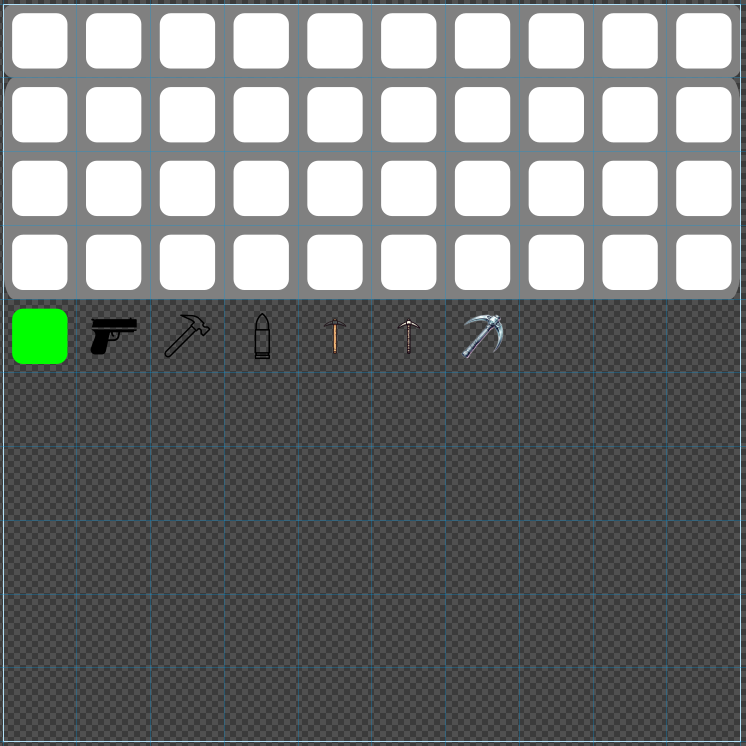
\includegraphics[width=0.8\textwidth]{chapters/two_dimensional_graphics/resources/SpriteSheet.png}
    \caption{Inventory Sprite Sheet}
    \label{fig:inventory}
\end{figure}
    
\begin{figure}[H]
    \begin{lstlisting}[language=json,firstline=1]
    {
        "width": 10,
        "height": 10,
        "items": [
            {
            "name": "hotbar",
            "x": 0,
            "y": 0,
            "width": 10,
            "height": 1
            },
        ]
    }
    \end{lstlisting}

    \caption{Inventory Sprite Sheet JSON}
    \label{lst:inventory_sprite_sheet_json}
\end{figure}
\subsection*{Heads Up Display} \label{sec:hud}
The HUD encapsulates all the 2d elements that are drawn on top of the 3d scene while the game is runnings.
This includes:
\begin{itemize}
    \item Crosshair
    \item FPS counter
    \item Player position
    \item Inventory
\end{itemize}

The Crosshair is a simple cross in the middle of the screen.
It is used to help the player aim.
It consists of 2 lines and does not use any textures.

The FPS counter is a simple text that shows the current FPS.
It is drawn in the top right corner of the screen.
It uses the symbols texture.

The player position is a simple text that shows the current position of the player.
It is drawn in the top left corner of the screen.
It uses the symbols texture.

The inventory is a collection of images that represent the items the player has.
It is drawn at the bottom of the screen.
It uses both the textures.
The images of the items are drawn first and then the text is drawn on top of them.
It is done in this order to optimize the performance by minimizing the number of times a texture is set to 2.

All the elements of the HUD have their own positions and sizes.
Each element is either placed in some position on the screen or is placed relative to some other element.
\subsection*{Menu} \label{sec:menu}
Menu is a lot more complicated than the HUD which is described in \autoref*{sec:hud}.
Because of that we decided to create a framework for creating menus.
This framework was heavily inspired by Flutter.
It uses the same concepts and terminology.
The overall idea is that everything is a widget.
A widget is a class that has a render method as well as a get size method.
The render method takes a context which includes information about the position and size on the screen that the widget can render to.
Some widgets also have children so the overall structure of the menu is a tree of widgets.

An example of a widget is shown in \autoref*{fig:main_menu}.
This widget renders the main menu of the game.
The rendering logic of this widget can be seen in \autoref*{fig:widget_logic}.
The idea is as follows.
The root widget calls the render method of it's child which is the \texttt{Background} widget.
The \texttt{Background} widget renders a background color.
Then the \texttt{Background} widget calls the render method of it's child which is the \texttt{Column} widget.
This widget renders it's children in a column but to do that it first needs to know the size of each of its children.
Based on that information it will call a render method of each child with the appropriate context.
Each child asks it's children for their size recursively until it reaches a leaf widget.
The process stops at the leaf and the render method is called on the children of the column widget.

This is a simplified version of the rendering logic as each widget has multiple options and rules that change how it or it's children are rendered.
For example, the \texttt{Column} widget has a \texttt{alignment} property which changes how the children are aligned.
The \texttt{Button} widget in the \autoref*{fig:widget_logic} itself is a tree of widgets.

This approach of rendering the menu is very flexible and allows for a lot of customization.
It improves on the method used to render the HUD described in \autoref*{sec:hud}.
This approach is not common in game development.
Usually menus are created by putting elements on the screen at specific positions. % TODO: cite something
In this part we believe that our approach is better than the traditional one and improves on approaches used in most popular game engines like Unity or Godot.

\begin{figure}[H]
    \centering
    \begin{minipage}{0.45\textwidth}
        \centering
        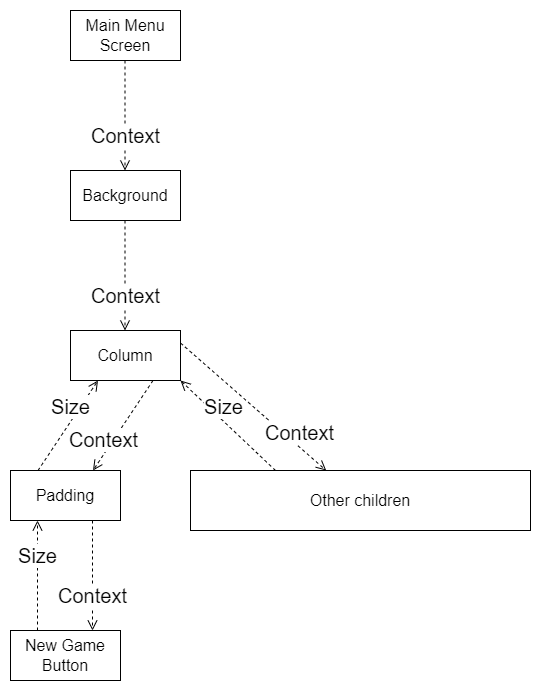
\includegraphics[width=0.8\textwidth]{chapters/two_dimensional_graphics/resources/widget_logic.drawio.png}
        \caption{Widget rendering logic.}
        \label{fig:widget_logic}
    \end{minipage}\hfill
    \begin{minipage}{0.45\textwidth}
        \centering
        \includegraphics[width=0.8\textwidth]{chapters/two_dimensional_graphics/resources/main-menu.png}
        \caption{Main menu.}
        \label{fig:main_menu}
    \end{minipage}
\end{figure}
\section*{Terrain Generation}
When designing the way the terrain is randomly generated so that we can have a new, unique map every time we play.
The second thing we wanted was to make sure that the player could edit the terrain in any way they wanted.
These two requirements made us decide on the algorithm described in this section.

The algorithm consists of the following steps:
\begin{itemize}
    \item Generate a scalar field for the whole world.
    \item Divide the world into chunks.
    \item Generate the terrain.
\end{itemize}

Each of these steps will be described in more detail alter in this section.

\subsection*{Scalar Field} \label{subsec:scalar_field}
The first step in the terrain generation is to generate a scalar field which is a function that takes a point in 3D space and returns a value.
What is important is that this function always returns the same value for the same point.
Another important feature is that the function should return close values for close points.
Our function returns values for points which have integer coordinates.

Having these properties in mind we decided to use the Perlin noise function.
Perlin noise first introduced by Ken Perlin in 1983 \cite{perlin_noise} is often used in computer graphics and in particular in procedural terrain generation.
It is a pseudo-random function that returns random values any point in 3D space.
However unlike other random functions it returns similar values for similar points.
This makes it ideal for this game.

The Perlin noise function is used to generate a value for each point in the scalar field.
This value is then modified based on 5 parameters: octaves, initial frequency, frequency multiplier, initial amplitude and amplitude multiplier.
These parameters are generate based on the seed of the world from 5 different sets of options which gives the game 5 terrains.
However we need more than just the value for each point.
Each point is also assigned a type based on the position that is later used to determine the type of the block which in turn determines its color.
The color
\subsection*{Chunks}
As mentioned before one of the most important thinks for the terrain was a way to edit it.
Editing the whole terrain at once would be very slow and not very efficient.
Thus the terrain is split into chunks - cubes with side length 16.
Each chunk is a separate object and can be edited independently.
This solution is much more efficient but is also has some problems.

One problem is that the terrain is not continuous.
Every time we edit a chunk we need to make sure that the edges of the chunk are the same as the edges of the neighboring chunks.
This is done by making sure that when a function that updates one chunk is called it is also called with the exact same parameters for other affected chunks.
Without this the terrain would have holes in it between chunks which is shown in a screenshot from an early version of the game in \autoref*{fig:gaps_between_chunks}.

Another problem is that the algorithm we used for generating the terrain, described in \autoref*{subsec:marching_cubes}, calculates normal vectors based on the values of the scalar field around the point at which the normal is calculated.
This means that that the normal vectors at the edges of the chunks have to be calculated differently.
This is a common problem with the algorithm and it is visualized in \autoref*{fig:problem_with_normals_at_chunk_edge}.
The most common solution and the one we used is extending the scalar field by one layer of points around the chunk.
This means that the chunk contains the information about the scalar field outside of the chunk itself.
That way the normal vectors can be calculated the same way for all points in the chunk.

\begin{figure}[H]
    \centering
    \begin{minipage}{0.45\textwidth}
        \centering
        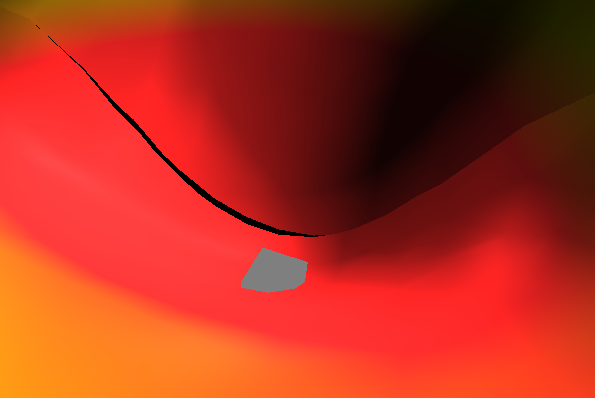
\includegraphics[width=0.8\textwidth]{chapters/terrain_generation/resources/chunk_edges_gaps.png}
        \caption{Gaps between chunks.}
        \label{fig:gaps_between_chunks}
    \end{minipage}\hfill
    \begin{minipage}{0.45\textwidth}
        \centering
        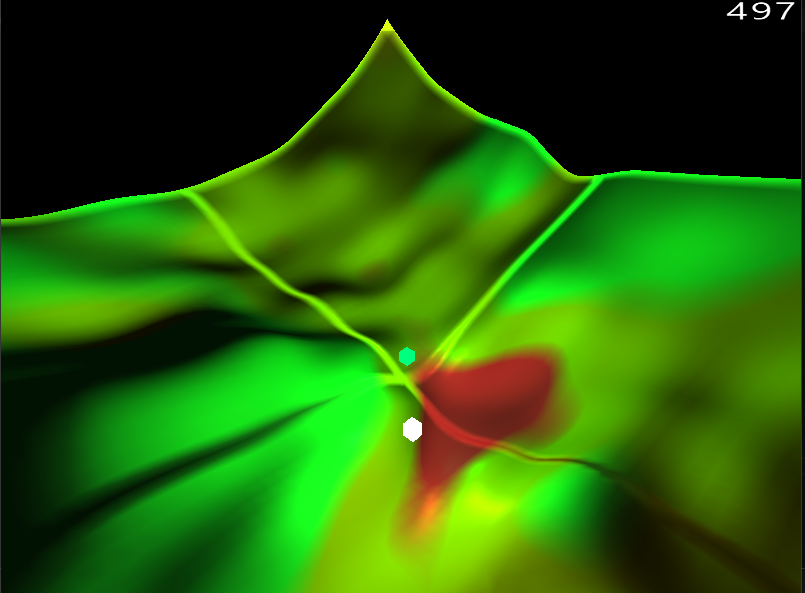
\includegraphics[width=0.8\textwidth]{chapters/terrain_generation/resources/chunk_edges_normals_problem.png}
        \caption{Problem with normals at chunk edges.}
        \label{fig:problem_with_normals_at_chunk_edge}
    \end{minipage}
\end{figure}
\subsection*{Marching Cubes} \label{subsec:marching_cubes}
Marching cubes is an algorithm for generating a 3D mesh from a scalar field.
It was first described by William E. Lorensen and Harvey E. Cline in 1987 \cite{marching_cubes}.
The main idea behind the algorithm is to divide the scalar field into cubes and then generate a mesh for each one of them.

Some isolevel is chosen and then each point that has a value greater than the isolevel is considered to be "above" the surface and each point with a value lower than the isolevel is considered to be "below" the surface.
We know that a surface has to separate the points that are above it from the points that are below it.
Every cube has 8 vertices and each vertex is either above or below the surface which gives us a total of 256 combinations (some combinations being rotations of others).
For each of these combinations we use a precomputed table to generate a mesh.
The table tells us which edges of the cube are intersected by the surface and how to connect them.
To make the mesh look smoother we interpolate the position of the vertices on the edges based on the values of the scalar field at the vertices.
This is done by using the linear interpolation. % Maybe add formula here?
This gives us a mesh.

However to make the mesh look even smoother we also need to calculate the normal vectors for each vertex.
The normal vectors for each vertex of the scalar field are calculated using \autoref*{eq:normal_vector}
\begin{equation}
    \label{eq:normal_vector}
    n(x, y, z) = \begin{bmatrix}
        s(x + 1, y, z) - s(x - 1, y, z) \\
        s(x, y + 1, z) - s(x, y - 1, z) \\
        s(x, y, z + 1) - s(x, y, z - 1)
      \end{bmatrix}
\end{equation}
where $s$ is the scalar field and $n$ is the normal vector.
These vectors are used to calculate the mesh normals using the same interpolation used for the mesh.

Last part of creating the mesh is assigning the colors to each vertex.
Each vertex of the scalar field is assigned a type which is described in \autoref*{subsec:scalar_field}.
Each type has a color assigned to it.
The color of each vertex of the mesh is calculated by interpolating the colors of the vertices of the scalar field.



\chapter{User Manual}\label{ch:user_manual}
This section describes how to launch and later use the application.
The user controls were made with industry standards in mind, so the user should not have any problems with using them.
However, if the user does not have much experience with video games, this section will help them get started as it provides a detailed start-to-finish description of how to play the game.

\section{Launching the game}
The application starts in the main menu shown in \autoref{fig:main_menu}.
From here a new game can be started, a previous save can be loaded, or a save can be deleted.
The user can also view controls, and exit the game.
To start a game for the first time, the user has to click on the "New Game" button which will show the "New Game Screen".

When the game is running the user can press the \keys{\escwin} key to show the main menu or hide it.
While the game is running the main menu will also show a "Resume" button which will resume the game and hide the menu.

\begin{figure}[H]
    \centering
    \includegraphics[width=0.8\textwidth]{chapters/user_manual/resources/main-menu.png}
    \caption{Main menu}
    \label{fig:main_menu}
\end{figure}
\section{New Game Screen}
The game can be started from the New Game screen shown in \autoref{fig:new_game}.
To start a game, the user has to click on the "Input Game Name" input text box.
This will allow them to enter a name for the game.
If there is no game save with the same name, the text box will light up green.
If there is already a game save with the same name, the text box will light up red.
If the box is green, the user can press one of the buttons to start a new game in the chosen geometry.

\begin{figure}[!htb]
    \centering
    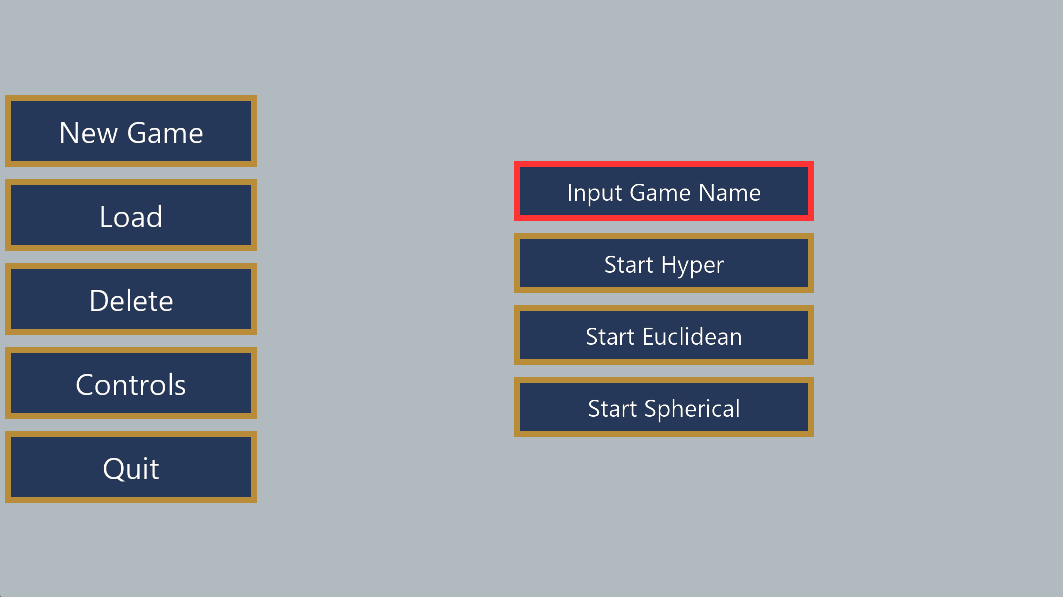
\includegraphics[width=0.8\textwidth]{chapters/user_manual/resources/new-game-no-input.png}
    \caption{New Game screen}
    \label{fig:new_game}
\end{figure}
\section{Load Game Screen}
The game can be loaded from the Load Game screen shown in \autoref{fig:load_game}.
This screen displays your 9 most recent saves.
The user can load a save by clicking a tile corresponding to the save.
To load a more recent save the user has to first delete more recent saves using the "Delete Game" described in \autoref{delete_save_screen}

\begin{figure}[h]
    \centering
    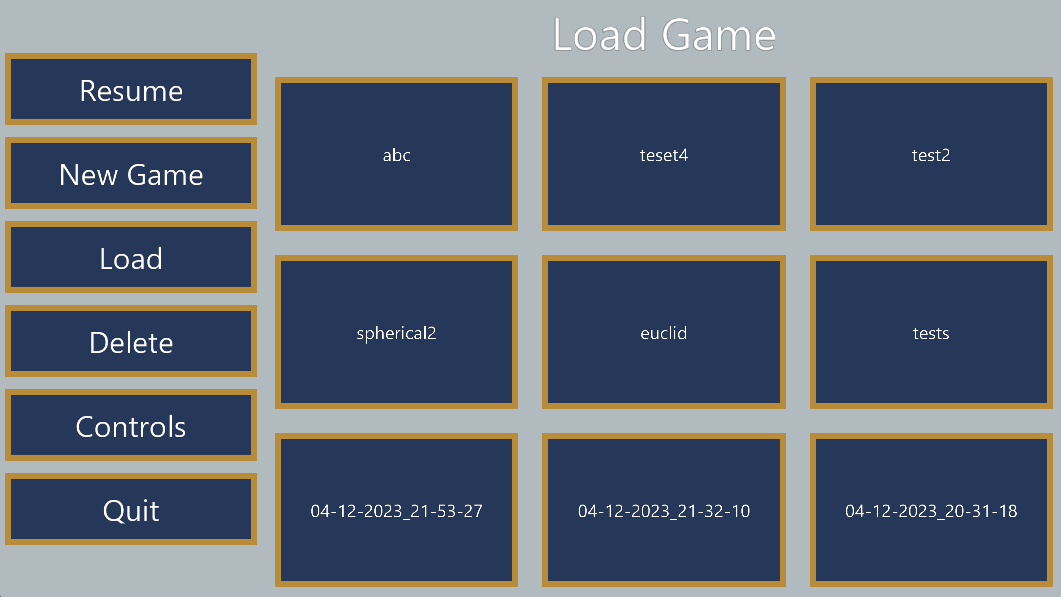
\includegraphics[width=0.8\textwidth]{chapters/user_manual/resources/load-game.png}
    \caption{Load Game screen}
    \label{fig:load_game}
\end{figure}
\subsubsection{Delete Save Screen} \label{delete_save_screen}
The "Delete Game" screen shown in \autoref{fig:delete_save} allows you to delete your saves.
It will display your 9 most recent saves.
To delete a save click on its name.
If a game is currently running you cannot delete its save.

\begin{figure}[H]
    \centering
    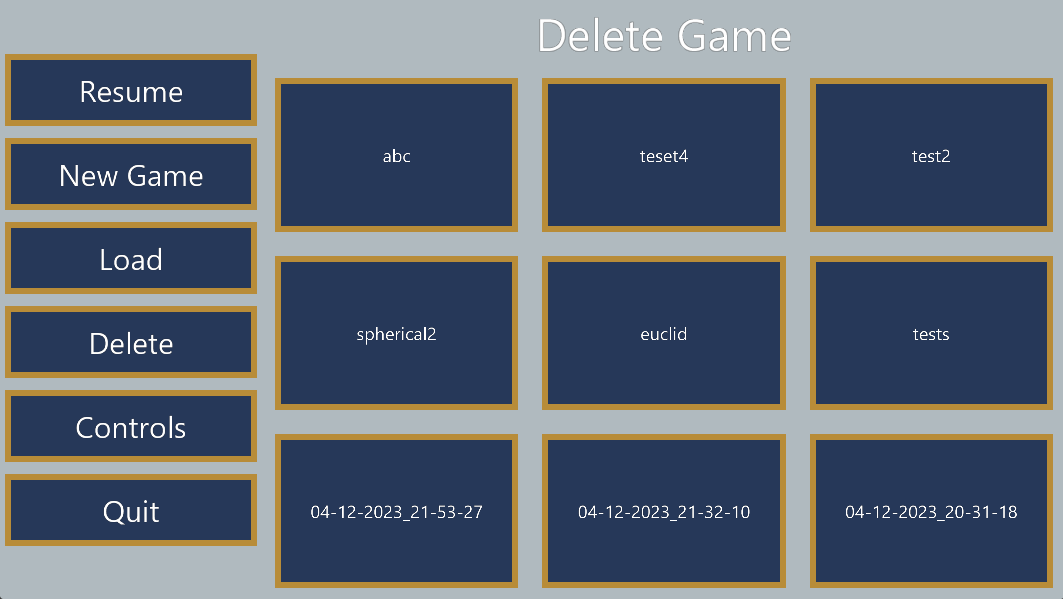
\includegraphics[width=0.8\textwidth]{chapters/user_manual/resources/delete-game.png}
    \caption{Delete Save screen}
    \label{fig:delete_save}
\end{figure}
\section{Controls}
The controls for the game are presented in \autoref{tab:game_key_functions}.
If the user forgets them, they can press the "Controls" button in the menu at any time to see them in the game, as shown in Figure \ref{fig:controls}.

\begin{table}[h]
    \centering
    \begin{tabular}{|m{3cm}|m{8cm}|}
        \hline
        \textbf{Key}              & \textbf{Function}                                              \\
        \hline
        \keys{W}                  & Move forward.                                                  \\
        \hline
        \keys{S}                  & Move back.                                                     \\
        \hline
        \keys{A}                  & Move left.                                                     \\
        \hline
        \keys{D}                  & Move right.                                                    \\
        \hline
        \keys{\shift}             & Sprint.                                                        \\
        \hline
        \keys{\SPACE}             & Jump.                                                          \\
        \hline
        \texttt{Left Mouse}       & Use item.                                                      \\
        \hline
        \texttt{Right Mouse}      & Use item's second ability.                                     \\
        \hline
        \keys{\escwin}            & Show/Hide menu.                                                \\
        \hline
        \keys{\tab}               & Switch camera between 1st and 3rd person.                      \\
        \hline
        \texttt{Scroll}           & Change curvature (works only in hyperbolic geometry).          \\
        \hline
        \keys{0} through \keys{9} & Select item.                                                   \\
        \hline
        \keys{C}                  & Enter car.                                                     \\
        \hline
        \keys{F}                  & Flip car (works only outside the car).                         \\
        \hline
        \keys{L}                  & Leave car.                                                     \\
        \hline
        \keys{Y}                  & Toggle flashlight/Toggle car reflectors (when inside the car). \\
        \hline
        \keys{F1}                 & Toggle cinematic mode.                                         \\
        \hline
        \keys{F3}                  & Toggle showing hitboxes.                                       \\
        \hline
    \end{tabular}
    \caption{Keyboard Key Functions for Game Controls}
    \label{tab:game_key_functions}
\end{table}

\begin{figure}[H]
    \centering
    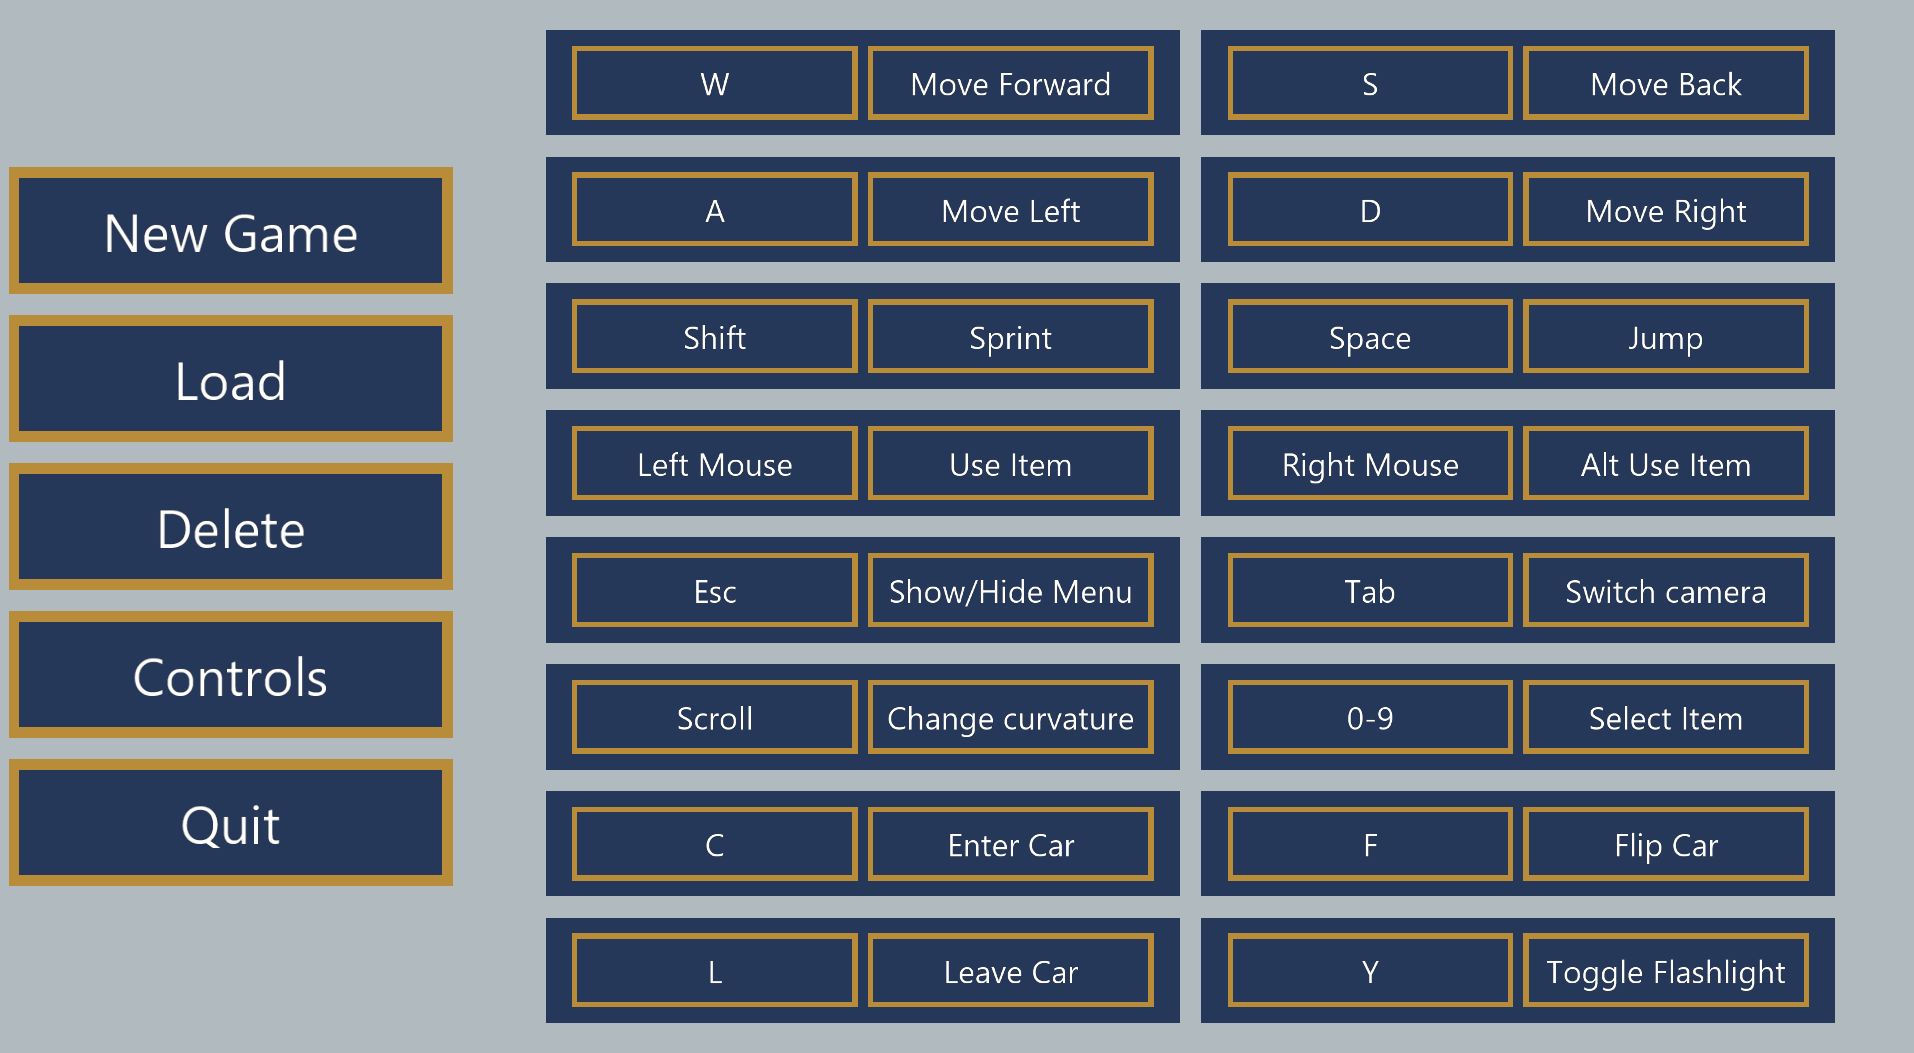
\includegraphics[width=0.8\textwidth]{chapters/user_manual/resources/controls.png}
    \caption{Controls screen}
    \label{fig:controls}
\end{figure}
\section{Items}
Items are a big part of the game.
Different items in the game have different uses.
Description of all the in-game items can be found in \autoref{tab:mytable}.
To use the items the player has to first select the desired item using number keys \keys{0} through \keys{9}.
The selected item will be highlighted in the inventory as shown in \autoref{fig:inventory}, in which the selected item is the gun.
The player can use the item by pressing the left mouse button (\texttt{LMB}) or the right mouse button (\texttt{RMB}).
The effect of the item depends on the item itself and the mouse button used.

\begin{table}[h]
    \centering
    \begin{tabular}{|c|p{5cm}|p{5cm}|}
        \hline
        Item                                                                         & \texttt{LMB} Effect                                                                   & \texttt{RMB} Effect \\
        \hline
        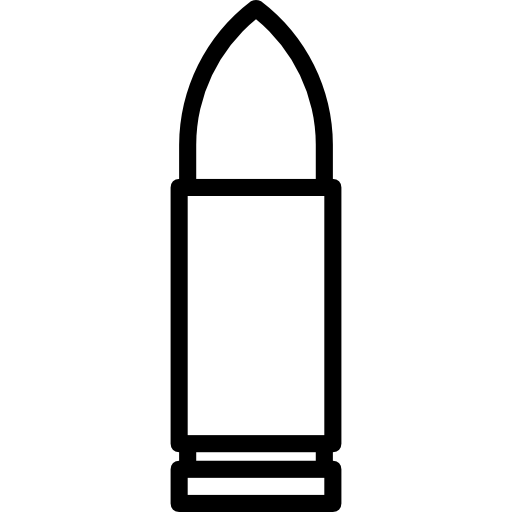
\includegraphics[width=1cm]{chapters/user_manual/resources/bullet.png}       & No effect                                                                             & No effect           \\
        \hline
        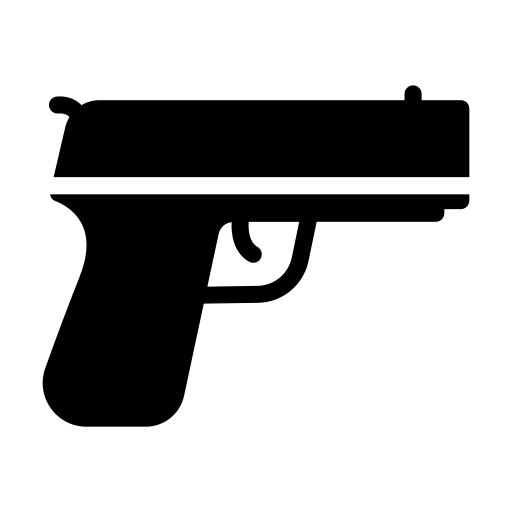
\includegraphics[width=1cm]{chapters/user_manual/resources/pistol.png}       & Fires a bullet if there is one in the inventory. Removes a bullet from the inventory. & No effect           \\
        \hline
        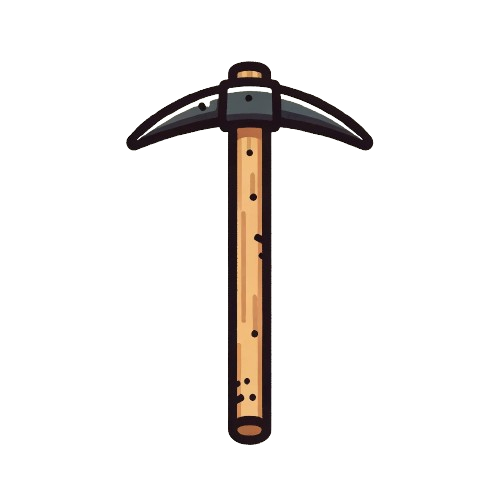
\includegraphics[width=1cm]{chapters/user_manual/resources/pickaxe-slow.png} & Mines slowly.                                                                         & Builds slowly.      \\
        \hline
        
\includegraphics[width=1cm]{chapters/user_manual/resources/pickaxe-mid.png}  & Mines.                                                                                & Builds.             \\
        \hline
        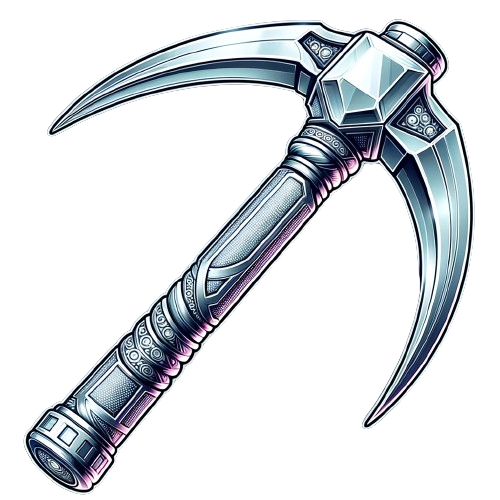
\includegraphics[width=1cm]{chapters/user_manual/resources/pickaxe-fast.png} & Mines quickly.                                                                        & Builds quickly.     \\
        \hline
    \end{tabular}
    \caption{Table of in game items}
    \label{tab:mytable}
\end{table}

\begin{figure}[H]
    \centering
    
\includegraphics[width=0.8\textwidth]{chapters/user_manual/resources/inventory.png}
    \caption{Inventory}
    \label{fig:inventory}
\end{figure}
\section{Gameplay}\label{sec:gameplay}
After the game is started, the user can finally start playing.
At the start, the screen will look like in \autoref{fig:gameplay}.
The user can see their position in the top left corner, the current frames per second in the top right corner, and the inventory in the bottom of the screen.
In the middle of the screen, there is a crosshair that shows where the user is aiming.
The user can also see their character model.
By using the controls described in \autoref{sec:controls}, the user can start moving around and exploring the world.


\begin{figure}[h]
    \centering
    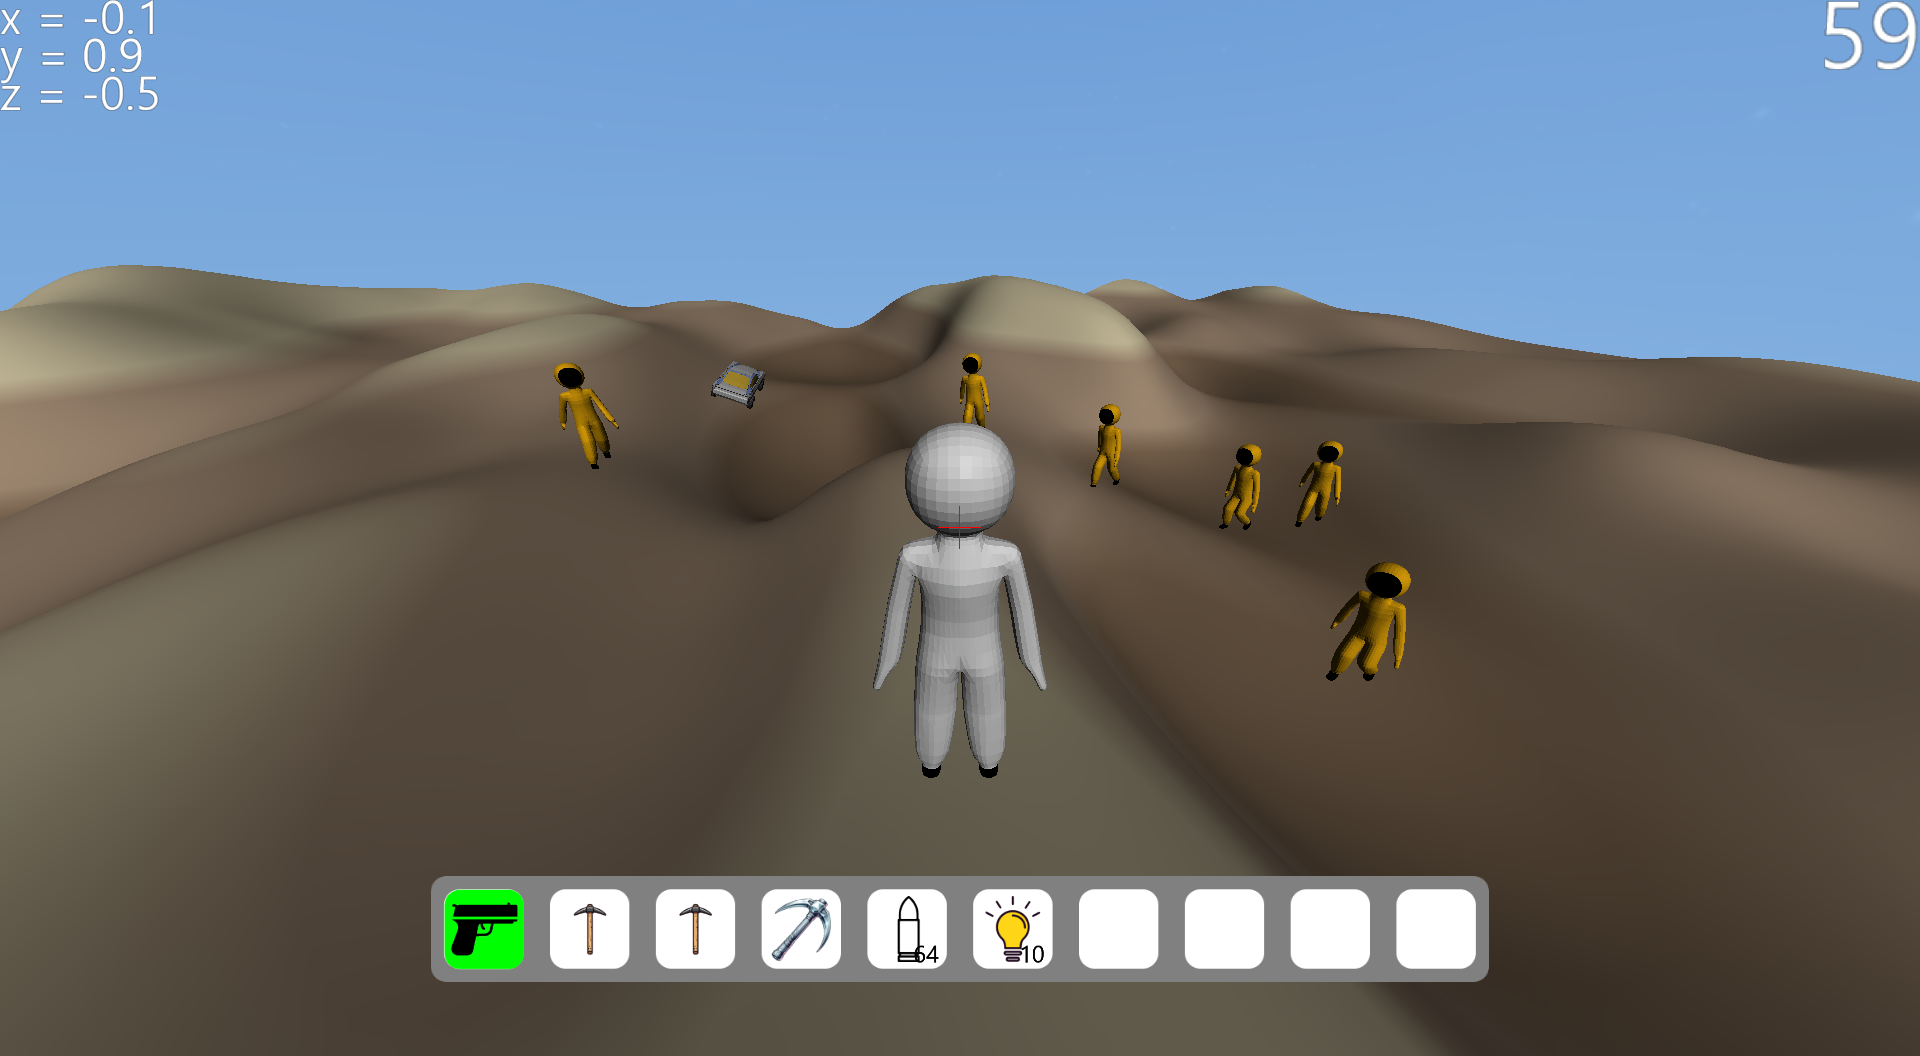
\includegraphics[width=0.8\textwidth]{chapters/user_manual/resources/gameplay.png}
    \caption{Controls screen}
    \label{fig:gameplay}
\end{figure}

% ------------------------------- BIBLIOGRAPHY ---------------------------
% LEXICOGRAPHICAL ORDER BY AUTHORS' LAST NAMES
% FOR AMBITIOUS ONES - USE BIBTEX


\begin{thebibliography}{20} % IF YOU HAVE MORE REFERENCES, WRITE THE BIGGER NUMBER

  \bibitem[1]{Ktos} A. Author, \emph{Title of a book}, Publisher, year, page--page.
  \bibitem[2]{Innyktos} J. Bobkowski, S. Dobkowski, Title of an article, \emph{Magazine X, No. 7}, year, PAGE--PAGE.
  \bibitem[3]{B} C. Brink, Power structures, \emph{Algebra Universalis 30(2)}, 1993, 177--216.
  \bibitem[4]{H} F. Burris, H. P. Sankappanavar, \emph{A Course of Universal Algebra}, Springer-Verlag, New York, 1981.
\end{thebibliography}
\pagenumbering{gobble}
\thispagestyle{empty}



% ----------------------- LIST OF SYMBOLS AND ABBREVIATIONS ------------------
\chapter*{List of symbols and abbreviations}

\begin{tabular}{cl}
  nzw.           & nadzwyczajny  \\
  *              & star operator \\
  $\widetilde{}$ & tilde
\end{tabular}
\\
If you don't need it, delete it.
\thispagestyle{empty}


% ----------------------------  LIST OF FIGURES --------------------------------
\listoffigures
\thispagestyle{empty}
If you don't need it, delete it.


% -----------------------------  LIST OF TABLES --------------------------------
\renewcommand{\listtablename}{Spis tabel}
\listoftables
\thispagestyle{empty}
If you don't need it, delete it.

% -----------------------------  LIST OF APPENDICES ---------------------------
\chapter*{List of appendices}
\begin{enumerate}
  \item Appendix 1
  \item Appendix 2
  \item In case of no appendices, delete this part.
\end{enumerate}
\thispagestyle{empty}


\end{document}
